% see http://info.semprag.org/basics for a full description of this template
\documentclass[charis]{glossa}

% possible options:
% [times] for Times font (default if no option is chosen)
% [cm] for Computer Modern font
% [lucida] for Lucida font (not freely available)
% [brill] open type font, freely downloadable for non-commercial use from http://www.brill.com/about/brill-fonts; requires xetex
% [charis] for CharisSIL font, freely downloadable from http://software.sil.org/charis/
% for the Brill an CharisSIL fonts, you have to use the XeLatex typesetting engine (not pdfLatex)
% [biblatex] for using biblatex
% [linguex] loads the linguex example package
% !! a note on the use of linguex: in glossed examples, the third line of the example (the translation) needs to be prefixed with \glt. This is to allow a first line with the name of the language and the source of the example. See example (2) in the text for an illustration.
% !! a note on the use of bibtex: for PhD dissertations to typeset correctly in the references list, the Address field needs to contain the city (for US cities in the format "Santa Cruz, CA")

\title[]{An exploratory study of voicing-related differences in vowel duration as
compensatory temporal adjustment in Italian and Polish}

% \author[Paul \& Vanden Wyngaerd]% short form of the author names for the running header. If no short author is given, no authors print in the headers.
% {%as many authors as you like, each separated by \AND.
%   \spauthor{Waltraud Paul\\
%   \institute{CNRS, CRLAO}\\
%   \small{105, Bd. Raspail, 75005 Paris\\
%   waltraud.paul@ehess.fr}
%   }
%   \AND
%   \spauthor{Guido Vanden Wyngaerd \\
%   \institute{KU Leuven}\\
%   \small{Warmoesberg 26, 1000 Brussel\\
%   guido.vandenwyngaerd@kuleuven.be}
%   }%
% }

\author[]{
  }

\usepackage{natbib}


\usepackage{cleveref}
\usepackage{ctable}
\usepackage{enumerate}
\usepackage{lineno}
\linenumbers

\begin{document}

\sffamily
\maketitle




\rmfamily

%  Body of the article
\begin{abstract}
  Over a century of phonetic research has established the cross-linguistic existence of the so called `voicing effect', by which vowels tend to be shorter when followed by voiceless stops and longer when the following stop is voiced.
  However, no agreement is found among scholars regarding the source of this effect, and several causal accounts have been advanced.
  A notable one is the compensatory temporal adjustment account, according to which the duration of the vowel is inversely correlated with the stop closure duration (voiceless stops having longer closure durations than voiced stops).
  The compensatory account has been criticised due to lack of empirical support and its vagueness regarding the temporal interval within which compensation is implemented.
  The results from this exploratory study of Italian and Polish suggest that the duration of the interval between two consecutive stop releases in CVCV words in these languages is not affected by the voicing of the second stop.
  The durational difference of the first vowel then would follow from differences in closure durations of the following stop.
  While other factors (like perceptual biases) could also play a role in the development of the voicing effect, the data discussed here shed new light on a possible production account of voicing-related differences in vowel durations.
\end{abstract}

\section{Introduction}\label{introduction}

\label{s:intro}

Almost a hundred years of research have consistently shown that
consonantal voicing has an effect on preceding vowel duration: vowels
followed by voiced obstruents are longer than when followed by voiceless
ones (\citealt{meyer1904}; \citealt{heffner1937}; \citealt{house1953};
\citealt{belasco1953}; \citealt{peterson1960}; \citealt{halle1967};
\citealt{chen1970}; \citealt{klatt1973}; \citealt{lisker1974};
\citealt{laeufer1992}; \citealt{fowler1992}; \citealt{hussein1994};
\citealt{lampp2004}; \citealt{warren2005}; \citealt{durvasula2012}).
This so called `voicing effect' has been found in a considerable variety
of
languages.\footnote{One of the first attestations of the term `voicing effect' can be attributed to \citet{mitleb1982}. Probably \citet{wells1990} introduced the term `pre-fortis clipping', which can also be found in the literature.}
These include (but are not limited to) English, German, French, Spanish,
Hindi, Russian, Italian, Arabic, and Korean (see \citealt{maddieson1976}
for a more comprehensive, but still not exhaustive
list).\footnote{A typological note: Most languages reported having a voicing effect come from the Indo-European family. Others are from a pool of widely studied languages. It is thus of vital importance that future studies look at other language families and underdocumented/underdescribed languages.}
Despite of the plethora of evidence in support of the \emph{existence}
of the voicing effect, agreement hasn't been reached regarding its
\emph{source}.

Several proposals have been put forward in relation to the possible
source of the voicing effect (see \citealt{soskuthy2013} and
\citealt{begus2017} for an overview). Some of the proposed accounts
place the source of the voicing effect in properties of speech
production. A notable production account, which will be the focus of
this study, is the compensatory temporal adjustment account
\citep{lindblom1967, slis1969a, slis1969, lehiste1970, lehiste1970a}.
According to this account, the voicing effect follows from the
reorganisation of gestures within a unit of speech the duration of which
is not affected by stop voicing. The duration of such unit is held
constant across voicing contexts, while the duration of voiceless and
voiced obstruents differs. The closure of voiceless stops is longer than
that of voiced stops
\citep{lisker1957, van-summers1987, davis1989, de-jong1991}. As a
consequence, vowels followed by voiceless stops (which have a long
closure) are shorter than vowels followed by voiced stops (which have a
short closure). Advocates of the compensatory account propose two
prosodic units as the scope of the temporal adjustment: the syllable
(and, equivalently, the VC sequence ot vowel-to-vowel interval,
\citealt{lindblom1967, farnetani1986}), and the word
\citep{slis1969a, slis1969, lehiste1970, lehiste1970a}. However, the
compensatory temporal adjustment account has been criticised in
subsequent work.

Empirical evidence and logic challenge the proposal that the syllable or
the word have a constant duration and hence drive compensation. First,
Lindblom's \citeyear{lindblom1967} argument that the duration of the
syllable is constant is not supported by the findings in
\citet{chen1970} and \citet{jacewicz2009}. \citet{chen1970} rejects a
syllable-based compensatory account in the light of the fact that the
duration of the syllable is affected by consonant voicing.
\citet{jacewicz2009} further show that the duration of monosyllabic
words in American English changes depending on the voicing of the coda
consonant. Second, although the results in \citet{slis1969} suggest that
the duration of disyllabic words in Dutch is constant whether the second
stop is voiceless or voiced, it does not follow from this fact that
compensation should necessarily target the vowel preceding the stop.
Indeed, it is logically possible that the following unstressed vowel
could be the target of the compensation, therefore differences in
preceding vowel duration still call for an explanation.

The compensatory temporal adjustment account has been further challenged
on the basis of the so called `aspiration effect' \citep{maddieson1976},
by which vowels are longer when followed by aspirated stops than when
followed by unaspirated stops. In Hindi, vowels before voiceless
unaspirated stops are short, vowels followed by voiced aspirated stops
are long, and vowels followed by voiced unaspirated and voiceless
aspirated stops are in between and have similar durations.
\citet{maddieson1976} find no compensatory pattern between vowel and
consonant duration The consonant /t/, which has the shortest duration,
is preceded by the shortest vowel, and vowels before /d/ and /tʰ/ have
the same duration although the durations of the two consonants are
different. \citet{maddieson1976} argue that a compensatory explanation
for differences in vowel duration cannot be maintained.

However, a re-evaluation of the way consonant duration is measured in
\citet{maddieson1976} might actually turn their findings in favour of a
compensatory account. Due to difficulties in detecting the release of
the consonant of interest, consonant duration in \citet{maddieson1976}
is measured from the closure of the relevant consonant to the release of
the following, (e.g., in \emph{ab sāth kaho}, the duration of /tʰ/ in
\emph{sāth} is calculated as the interval between the closure of /tʰ/
and the release of /k/). This measure includes the burst and aspiration
(if present) of the consonant following the target vowel.
\citet{slis1969a}, however, state that the inverse relation between
vowel duration and the following consonant applies to \textit{closure}
duration, and not to the entire \textit{consonant}
duration.\footnote{In this paper, I use the term \textit{relation} to mean a categorical pattern of entailment (like in `a long vowel entails a short closure'), while the term \textit{correlation} is reserved to a statistical correlation of two continuous variables.}
If an inverse relation exists between vowel and closure duration, the
inclusion of burst and/or aspiration clearly alters this relationship.

Indeed, the study on Hindi voicing and aspiration effects conducted by
\citet{durvasula2012} indicates that closure duration, measured from
closure onset to closure offset, decreases according to the hierarchy
voiceless unaspirated \textgreater{} voiced unaspirated \textgreater{}
voiceless aspirated \textgreater{} voiced aspirated, which closely
resembles the order of increasing vowel duration in
\citet{maddieson1976}. Nonetheless, \citet{durvasula2012} do not find a
negative correlation between vowel duration and consonant closure
duration, but rather a (small) \emph{positive effect}. Vowel duration
increases with closure duration when voicing and aspiration are taken
into account. However, as noted in \citet{begus2017}, it is likely that
this result is a consequence of not controlling for speech rate. A small
negative effect of closure duration can turn positive if the effect of
speech rate (which is positive) is greater, given the cumulative nature
of these effects \citep[p. 2177]{begus2017}.

\citet{de-jong1991} finds partial support for a compensatory mechanism
between vowel and closure duration in an electro-magneto-articulometric
study of two American English speakers. The duration of vowels in
nuclear accented, pre-, and post-nuclear accented position is weakly
negatively correlated with closure duration (the slope coefficients
range between -0.12 and -0.35, meaning that the amount of durational
compensation is between 10\% and 35\%). Although it is difficult to draw
definite conclusions based on the data of two speakers, and while the
magnitude of the correlation is quite weak to univocally support
compensation, the direction of the correlation is correct (i.e.~a
negative correlation).

Further evidence for a compensatory account and a negative correlation
between vowel and closure duration comes from the effect of a third type
of consonants, namely ejectives. \citet{begus2017} finds that in
Georgian (which contrasts aspirated, voiced, and ejective consonants)
vowels are short when followed by voiceless aspirated stops, longer
before ejective stops, and longest when followed by voiced stops.
Crucially, stop closure duration follows the reversed pattern: closure
is short in voiced stops, longer in ejectives, and longest in voiceless
aspirated stops. Moreover, vowel duration is inversely correlated with
closure across the three phonation types. \citet{begus2017} mentions the
possibility that the negative correlation is an artefact of the vowel
and closure intervals sharing a boundary. This annotation bias could
generate negative correlations (by which the vowel would shorten and the
closure would lengthen by the same amount when, for example, the
boundary is placed to the left of the `actual' boundary). However, Beguš
shows with a cross-annotator analysis that this was not the case.
Moreover, I would like to add that, if misplacement of the V-C boundary
is due to random error (which is a neutral assumption to make), the
measured displacement from the `actual' boundary will approximately
follow a normal distribution with mean 0. \citet{begus2017} argues that
these findings support a temporal compensation account (although not
univocally, see \citealt[Section V]{begus2017}).

To summarise, a compensatory temporal adjustment account has been
proposed as the pathway to the emergence of the voicing effect.
According to such account, the difference in vowel duration before
consonants varying in voicing (and possibly other phonation types) is
the outcome of a compensation between vowel and closure duration. After
reviewing the critiques advanced by \citet{chen1970} and
\citet{maddieson1976}, and in face of the results in \citet{slis1969},
\citet{de-jong1991} and \citet{begus2017}, a temporal compensation
account gains credibility. However, issues about the actual
implementation of the compensation mechanism still remain. In
conclusion, while the compensatory temporal adjustment account is
plausible on the light of the reviewed literature, we are still left
with the necessity of identifying a speech interval the duration of
which is not affected by the voicing of the post-vocalic consonant, and
within which compensation can be logically implemented.

\subsection{The present study}\label{the-present-study}

This paper reports on selected results from a broader exploratory study
that investigates the relationship between vowel duration and consonant
voicing from both an acoustic and articulatory perspective. Synchronised
recordings of audio, ultrasound tongue imaging, and electroglottography
were carried out to enable a data-driven approach to the analysis of
features related to the voicing effect in the context of disyllabic
(CV́CV) words in Italian and
Polish.\footnote{As per \citet{cysouw2013}, the glossonyms \textit{Italian} and \textit{Polish} as used here to refer, respectively, to the languoids Italian [\textsc{Glottocode}: \texttt{ital1282}] and Polish [\textsc{Glottocode}: \texttt{poli1260}].}
This study, in its exploratory nature, was not designed to test the
compensatory account, but rather to collect synchronised articulatory
and acoustic data on the voicing effect. Moreover, the design of the
study has been constrained by the use of ultrasound articulatory
techniques (see \Cref{s:method}). Since the tongue imaging and
electroglottographic data don't bear on the main argument put forward
here, only the results from acoustics will be discussed.

Italian and Polish reportedly differ in the magnitude (or presence) of
the effect of stop voicing on vowel duration, while they are both
classified as voicing languages (languages in which the laryngeal
opposition in consonants is between voiceless unaspirated and voiced
consonants,
\citealt{beckman2013}).\footnote{Note that, while Polish neutralises the voicing contrast word-finally, it is maintained word-medially.}
For this reason, these two languages offer the opportunity to
investigate differences that could reveal mechanisms underlying the
voicing effect. Moreover, given that Italian and Polish share---on a
general level---some features of the segmental and prosodic make-up of
their phonological systems, the design of the experimental material and
comparison of the results is facilitated.

Italian has been unanimously reported as a voicing-effect language
\citep{caldognetto1979, farnetani1986, esposito2002}. The mean
difference in vowel duration when followed by voiceless vs.~voiced
consonants ranges between 22 and 24 ms in these studies, with longer
vowels followed by voiced consonants. The mean differences are based on
3 speakers in \citealt{farnetani1986} and 7 speakers in
\citealt{esposito2002}. \citealt{caldognetto1979} does not report
estimates of vowel duration, just the direction of the effect, but the
study is based on 10 speakers. On the other hand, the results regarding
the presence and magnitude of the effect in Polish are mixed. While
\citet{keating1984} reports no effect of voicing on vowel duration in
data from 24 speakers, \citet{nowak2006} finds that vowels followed by
voiced stops are 4.5 ms longer in the 4 speakers recorded.
\citet{malisz2008} argue based on data from 40 speakers that the
magnitude of the voicing effect in Polish is highly idiosyncratic, and
claim that their results are inconclusive on this matter. While they do
not report estimates from the 40 speakers, a table with mean vowel
durations from 4 suggests a mean difference before voiceless vs.~voiced
stops of 3.5 ms.

The acoustic data from the exploratory study discussed here suggests
that (1) a voicing effect can be detected both in Italian and Polish,
and that (2) the duration of the interval between two consecutive stop
releases (the release to release interval) is not affected by the
voicing of the second consonant in both languages. This finding is
compatible with a compensatory temporal adjustment account by which the
timing of the closure onset of the stop following the vowel within said
interval determines the respective durations of vowel and closure.

\section{Method}\label{method}

\label{s:method}

\subsection{Participants}\label{participants}

For this exploratory study, a target of 10 speakers per language was
set. A low target number of participants was required to keep the time
needed for processing the ultrasound data at manageable levels, since it
generally requires more time than in more standard acoustic analysis.
The stopping rule for recruitment was to reach 10 speakers in both
languages or to end data collection within 15 months from the start.
This rule was chosen to comply with resources and time limits.
Participants were sought in Manchester (UK), and in Verbania (Italy).
Seventeen subjects in total participated in this study. Eleven subjects
are native speakers of Italian (5 female, 6 male), while six are native
speakers of Polish (3 female, 3 male). The Italian speakers are from the
North and Centre of Italy (8 speakers from Northern Italy, 3 from
Central Italy). The Polish group has 2 speakers from Western Poland, 3
speakers from Central Poland, and 1 speaker from Eastern Poland. For
more information on the sociolinguistic details of the speakers, see
\Cref{a:socioling}. Ethical clearance for this study was obtained from
the University of Manchester (REF 2016-0099-76). The participants signed
a written consent and received a monetary compensation of £10.

\subsection{Equipment}\label{equipment}

The acquisition of the audio signal was achieved with the software
Articulate Assistant Advanced™ (AAA, v2.17.2, \citealt{articulate2011})
running on a Hawlett-Packard ProBook 6750b laptop with Microsoft Windows
7. Audio recordings were sampled at 22050 Hz (16-bit) and saved in a
proprietary format (\texttt{.aa0}). A FocusRight Scarlett Solo
pre-amplifier and a Movo LV4-O2 Lavalier microphone were used for audio
recording. The microphone was placed at the level of the participant's
mouth on one side, at a distance of about 10 cm. The microphone was
clipped onto a metal headset worn by the participant, which was part of
the ultrasonic equipment.

\subsection{Materials}\label{materials}

\label{s:materials}

The target stimuli were disyllabic words with
C\textsubscript{1}V\textsubscript{1}C\textsubscript{2}V\textsubscript{2}
structure, where C\textsubscript{1} = /p/, V\textsubscript{1} = /a, o,
u/, C\textsubscript{2} = /t, d, k, g/, and V\textsubscript{2} =
V\textsubscript{1} (e.g. /pata/, /pada/, /poto/,
etc.).\footnote{Italian has both a mid-low [ɔ] and a mid-high [o] back vowel in its vowel inventory. These vowels are traditionally described as two distinct phonemes \citep{kramer2009}, although both their phonemic status and their phonetic substance are subject to a high degree of geographical and idiosyncratic variability \citep{renwick2016}. As a rule of thumb, stressed open syllables in Italian (like the ones used in this study) have [ɔː] (vowels in penultimate stressed open syllables are long) rather than [oː] \citep{renwick2016}. On the other hand, Polish has only a mid-low back vowel phoneme /ɔ/ \citep{gussmann2007}. For sake of typographical simplicity, the symbol /o/ will be used here for both languages.}
Most are nonce words, although inevitably some combinations produce real
words both in Italian (4 words) and Polish (2 words, see
\Cref{a:targets}). The lexical stress of the target words was placed by
speakers of both Italian and Polish on V\textsubscript{1}, as intended.

The make-up of the target words was constrained by the design of the
experiment, which included ultrasound tongue imaging (UTI). Front vowels
are difficult to be imaged with UTI, since their articulation involves
tongue surface positions which are particularly far from the ultrasonic
probe, hence reducing the visibility of the tongue contour. For this
reason, only central and back vowels were included. Since one of the
variables of interest in the exploratory study was the closing gesture
of C\textsubscript{2}, only lingual consonants were used. A labial stop
was chosen as the first consonant to reduce possible coarticulation with
the following vowel (although see \citealt{vazquez-alvarez2007}). The
number of target words was kept low to reduce the time required for
completing the task, since the ultrasonic equipment can get very
uncomfortable for the speaker when worn for more than 15/20 minutes.

The target words were embedded in a frame sentence. Controlling for
meaning, segmental and prosodic make-up between languages proved to be
difficult. The frames are \emph{Dico X lentamente} `I say X slowly' in
Italian \citep[following][]{hajek2008}, and \emph{Mówię X teraz} `I say
X now' in Polish. These sentences were chosen in order to maintain a
similar intonation contour across languages.

\subsection{Procedure}\label{procedure}

The participant was asked to read the sentences with the target words
which were presented on the computer screen. The order of the sentences
was randomised for each participant. Participants read the list of
randomised sentence stimuli 6 times. Due to software constraints, the
order of the list was kept the same across the six repetitions within
each participant. The reading task lasted between 15 and 20 minutes,
with optional short breaks between one repetition and the other. The
total session time was around 45 minutes. Before the start of the
experiment, the participants were spoken to in their mother tongue to
try and reduce exposition to English prior to being recorded.
Instructions were also given in their respective mother tongues. Each
speaker read a total of 12 sentences for 6 times (with the exceptions of
IT02, who repeated the 12 sentences 5 times), which yields to a grand
total of 1212 tokens (792 from Italian, 420 from
Polish).\footnote{IT01 and IT02 (the first two participants of this study) also read sentences with words starting with /b/, which were later excluded from the experimental design. The data from /b/-initial words are not included in the analysis reported in this paper.}

The experiment was carried out in two locations: in the sound attenuated
booth of the Phonetics Laboratory at the University of Manchester
(directed by Dr.~Patrycja Strycharczuk), and in a quiet room in a field
location in Italy (Verbania, Northern Italy). In both locations the
equipment and procedures were the same. Data collection started in
December 2016 and ended in March 2018.

\subsection{Data processing and
measurements}\label{data-processing-and-measurements}

\ctable[caption = Criteria for the identification of acoustics landmarks,
label = t:dur-measures,
width=\textwidth,
star
]{ll>{\raggedright}p{9cm}}{}{
\FL
\textbf{landmark}               &                  & \textbf{criteria}                                                                                    \ML
vowel onset           & (V1 onset)         & Appearance of higher formants in the spectrogram following the release of /p/ (C1)            \NN
vowel offset          & (V1 offset)        & Disappearance of the higher formants in the spectrogram preceding the target consonant (C2) \NN
consonant onset       & (C2 onset)         & Corresponds to V1 offset                                                                    \NN
closure onset         & (C2 closure onset) & Corresponds to V1 offset                                                                    \NN
consonant offset      & (C2 offset)        & Appearance of higher formants of the vowel following C2 (V2); corresponds to V2 onset                                \NN
consonant release & (C1/C2 release)         & Automatic detection + manual correction \citep{ananthapadmanabha2014}                                           \LL
}

The audio recordings were exported from AAA in the \texttt{.wav} format
at the same sample and bit rate for further processing. A forced aligned
transcription was accomplished through the SPeech Phonetisation
Alignment and Syllabification software (SPPAS, \citealt{bigi2015}). The
outcome of the automatic annotation was manually corrected for the
relevant boundaries, according to the criteria in \Cref{t:dur-measures}
based on \citet{machac2009}. Segmentation boundaries not used in the
analyses have not been checked to speed up processing. The releases of
C1 and C2 were detected automatically by means of a Praat scripting
implementation of the algorithm described in
\citet{ananthapadmanabha2014}, and subsequently corrected if necessary.
The identification of the stop release was not possible in 99 tokens
(8\%) of C1 and 265 tokens (22\%) of C2 out of 1212. This was due either
to the absence of a clear burst in the waveform and spectrogram, or the
realisation of voiced stops as voiced fricatives. Most of the
fricativised tokens come from three speakers of Central Italian, IT12,
IT13, and IT14, a variety of Italian known to show processes of lenition
\citep{hualde2011}. Moreover IT12 and IT14 produced several tokens of
voiceless stops with voicing during closure (in some cases the closure
was completely voiced). These tokens have been used in the analyses,
because (1) the actual presence or absence of voicing during closure
does not bear on the compensatory account discussed here (which concerns
supraglottal gestures) and laryngeal gestures can be implemented almost
entirely independently from oral gestures, and (2) the voicing effect
has been shown to exist even in whispered speech, where vocal fold
vibration is entirely absent \citep{sharf1964}.

The durations in milliseconds of the following intervals were extracted
with a series of custom Praat scripts from the annotated acoustic
landmarks: word duration, vowel duration (V1 onset to V1 offset),
consonant closure duration (V1 offset to C2 release), and release to
release duration (C1 release to C2 release). Sentence duration was
measured in seconds. \Cref{f:segmentation} shows an example of the
segmentation of /pata/ (a) and /pada/ (b) from an Italian speaker.
Syllable rate (syllables per second) was used as a proxy to speech rate
\citep{plug2018a}, and was calculated as the number of syllables divided
by the duration of the sentence in seconds (8 syllables in Italian, 6 in
Polish). All further data processing and visualisation was done in R
v3.5.1 \citep{r-core-team2018, wickham2017}.

\begin{figure}
  \centering
  \subfigure[/pata/]{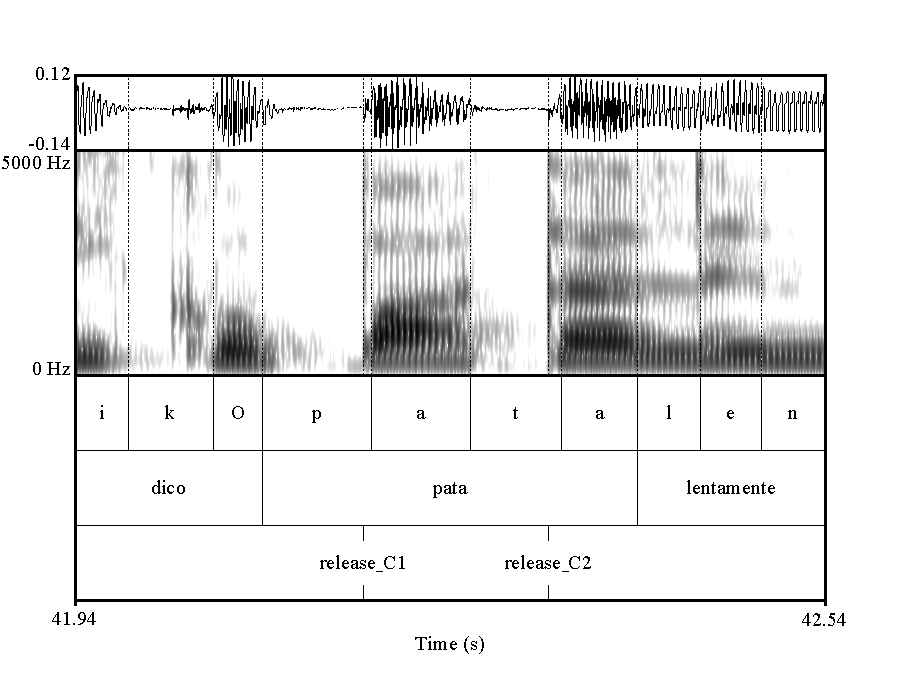
\includegraphics[height=2.5in]{img/Figure1a.pdf}}
  \subfigure[/pada/]{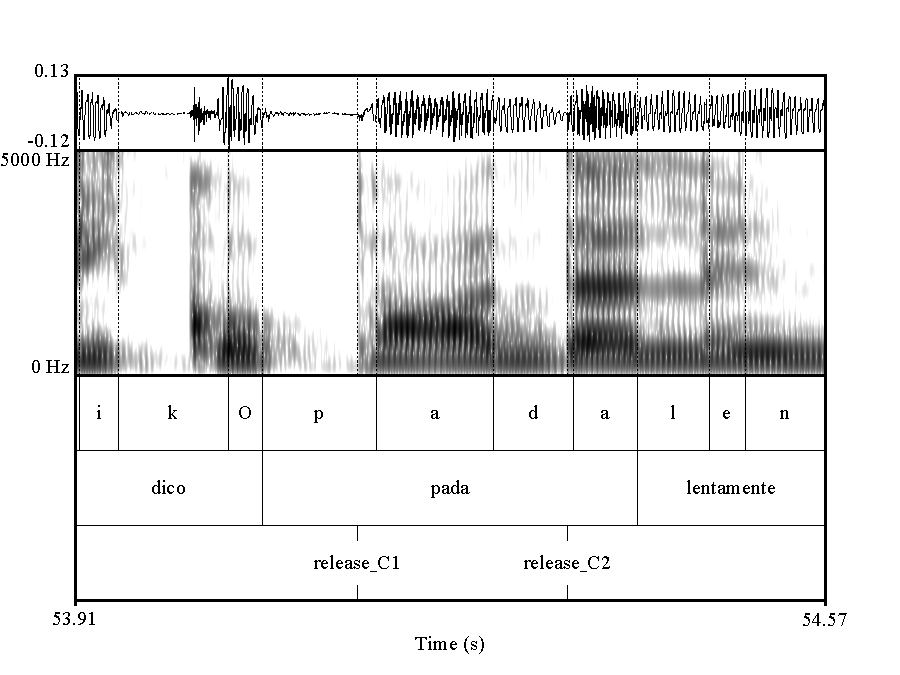
\includegraphics[height=2.5in]{img/Figure1b.pdf}}
  \caption{Segmentation example of the words \textit{pata} and \textit{pada} uttered by the Italian speaker IT09 (the times on the \textit{x}-axis refer to the times in the concatenated audio file)}
  \label{f:segmentation}
\end{figure}

\subsection{Statistical analysis}\label{statistical-analysis}

Given the data-driven nature of the study, all statistical analyses
reported here are to be considered exploratory (hypothesis-generating)
rather than confirmatory (hypothesis-driven,
\citealt{kerr1998, gelman2013, roettger2018}). The durational
measurements were analysed with linear mixed-effects models using
\texttt{lme4} v1.1-19 in R \citep{bates2015}, and model estimates were
extracted with the \texttt{effects} package v4.0-3 \citep{fox2003}. All
factors were coded with treatment contrasts and the following reference
levels: voiceless (vs.~voiced), /a/ (vs. /o/, /u/), coronal (vs.~velar),
Italian (vs.~Polish). Speech rate has been centred when included in the
models to make the intercept estimates more interpretable. The models
were fitted by Restricted Maximum Likelihood estimation (REML). The
estimates in the results section refer to these reference levels unless
interactions are discussed. \emph{P}-values for the individual terms
were obtained with \texttt{lmerTest} v3.0-1, which uses the
Satterthwaite's approximation to degrees of freedom
\citep{kuznetsova2017, luke2017}. A result is considered significant if
the \emph{p}-value is below the alpha level (\(\alpha = 0.05\)). The
choice of not using likelihood ratio tests for statistical inference is
based on \citet{luke2017} who argues that this approach can lead to
inflated Type I error rates. In any case, \citet[1501]{luke2017} also
warns that `results {[}from mixed-effects models{]} should be
interpreted with caution, regardless of the method adopted for obtaining
\textit{p}-values'.

Bayes factors were used to test whether word and release to release
duration are not affected by C2 voicing (i.e., the effect of C2 voicing
on duration is \texttt{0}). For each set of null/alternative hypotheses,
a full model (with the predictor of interest) and a null model
(excluding it) were fitted separately using the Maximum Likelihood
estimation (ML, \citealt[34]{bates2015}). The Bayes Information
Criterion (BIC) approximation was then used to obtain Bayes factors
\citep{raftery1995, raftery1999, wagenmakers2007, jarosz2014}. The
approximation is calculated according to the equation in \ref{eq:bayes}
\citep[796]{wagenmakers2007}.

\begin{equation}
\label{eq:bayes}
BF_{01} \approx exp(\Delta{}BIC_{10}/2)
\end{equation}

where \(\Delta{}BIC_{10} = BIC_1 - BIC_0\), \(BIC_1\) is the BIC of the
full model, and \(BIC_0\) is the BIC of the null model. Values of
\(BF_{01} > 1\) indicate a preference of H\textsubscript{0} over
H\textsubscript{1}. The interpretation of the Bayes factors follows the
recommendations in \citet[p.~139]{raftery1995}: 1--3 = weak evidence,
3--20 = positive evidence, 20--150 = strong evidence, \textgreater{} 150
= very strong evidence.

The extracted measurements were filtered before statistical analysis.
Measures of vowel duration, closure duration, word duration, and release
to release duration that are 3 standard deviations lower or higher than
the respective means were excluded from the final dataset (this
procedure generally corresponds to a loss of around 2.5\% of the data).
One sentence (sentence 48 of IT07, \emph{Dico pada lentamente}) included
a speech error and has been excluded. After excluding missing
measurements, these operations yield a total of 920 tokens of vowel and
closure durations, 1176 tokens of word duration, and 848 tokens of
release to release duration.

While the study has been devised to also allow comparison between
Italian and Polish, the low number of Polish speaker (6, against 11
Italian speakers) makes statistical comparison difficult (see
\citealt{kirby2018} and references therein for a discussion on
statistical power). The raw mean differences, presented in conjunction
with the estimates from statistical modelling, can still inform us on
the cross-linguistic differences and thus they will contribute to the
discussion of the results.

\subsection{Open Science statement}\label{open-science-statement}

Following recommendations for Open Science in \citet{cruwell2018} and
\citet{berez-kroeker2018} the data and code used to produce the analyses
discussed in this paper are available on the Open Science Framework at
\url{https://osf.io/bfyhr/?view_only=391ef2dcc2834039a90f739ddb6f137a}
\citep{coretta2018g}.

\section{Results}\label{results}

The following sections report the results of the study in relation to
the durations of vowels, consonant closure, word, and the release to
release interval. When discussing the output of statistical modelling,
only the relevant predictors and interactions will be presented. The
full output of statistical models (including confidence intervals and
\emph{p}-values) are given in \Cref{a:stats}.

\subsection{Vowel duration}\label{vowel-duration}

\label{s:vduration}

\begin{figure}
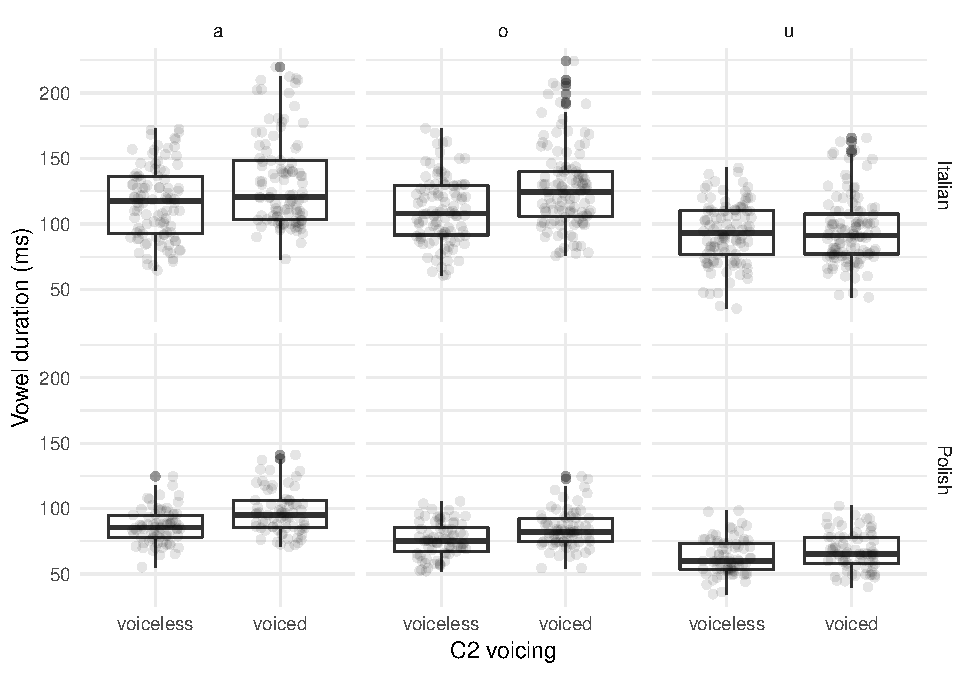
\includegraphics[width=\linewidth]{2018-relrel_files/figure-latex/Figure2} \caption{Raw data and boxplots of the duration in milliseconds of vowels in Italian (top row) and Polish (bottom row), for the vowels /a, o, u/ when followed by a voiceless or voiced stop}\label{f:Figure2}
\end{figure}

\Cref{f:Figure2} shows boxplots and raw data of vowel duration for the
three vowels /a, o, u/ when followed by voiceless or voiced stops in
Italian and Polish. Vowel tend to be longer when followed by a voiced
stop in both languages. The effect appears to be greater in Italian than
in Polish, especially for the vowels /a/ and /o/. There is no evident
effect of C2 voicing in /u/ in Italian, but the effect is discernible in
Polish /u/. In Italian, vowels have a mean duration of 106.16 ms (SD =
27.08) before voiceless stops, and a mean duration of 117.66 ms (SD =
34.63) before voiced stops. Polish vowels are on average 75.57 ms long
(SD = 16.16) when followed by a voiceless stop, and 83.11 ms long (SD =
19.37) if a voiced stop follows. The difference in vowel duration based
on the raw means is 11.5 ms in Italian and 7.54 ms in Polish.

A linear mixed-effects model with vowel duration as the outcome variable
was fitted with the following predictors: fixed effects for C2 voicing
(voiceless, voiced), C2 place of articulation (coronal, velar), vowel
(a, o, u), language (Italian, Polish), and speech rate (as syllables per
second, centred); by-speaker and by-word random intercepts with
by-speaker random slopes for C2 voicing. All possible interactions
between C2 voicing, vowel, and language were included. The following
terms are significant according to \emph{t}-tests with Satterthwaite's
approximation to degrees of freedom: C2 voicing, C2 place, vowel,
language, and speech rate. Only the interaction between C2 voicing and
vowel is significant. Vowels are 16.28 ms longer (SE = 4.42) when
followed by a voiced stop (C2 voicing), and 8 ms shorter (SE = 1.63)
when followed by a velar stop. The effect of C2 voicing is smaller with
/u/ (around 3 ms, \(\hat{\beta}\) = -13.1 ms, SE = 5.56). Polish has on
average shorter vowels than Italian (\(\hat{\beta}\) = -24.05 ms, SE =
7.83), and the effect of voicing is estimated to be about 10.55 ms
(although note that the interaction between language and C2 voicing is
not significant). Speech rate has a negative effect on vowel duration,
such that faster rates correlate with shorter vowel durations
(\(\hat{\beta}\) = -16.23 ms, SE = 1.26).

\subsection{Consonant closure
duration}\label{consonant-closure-duration}

\label{s:cduration}

\begin{figure}
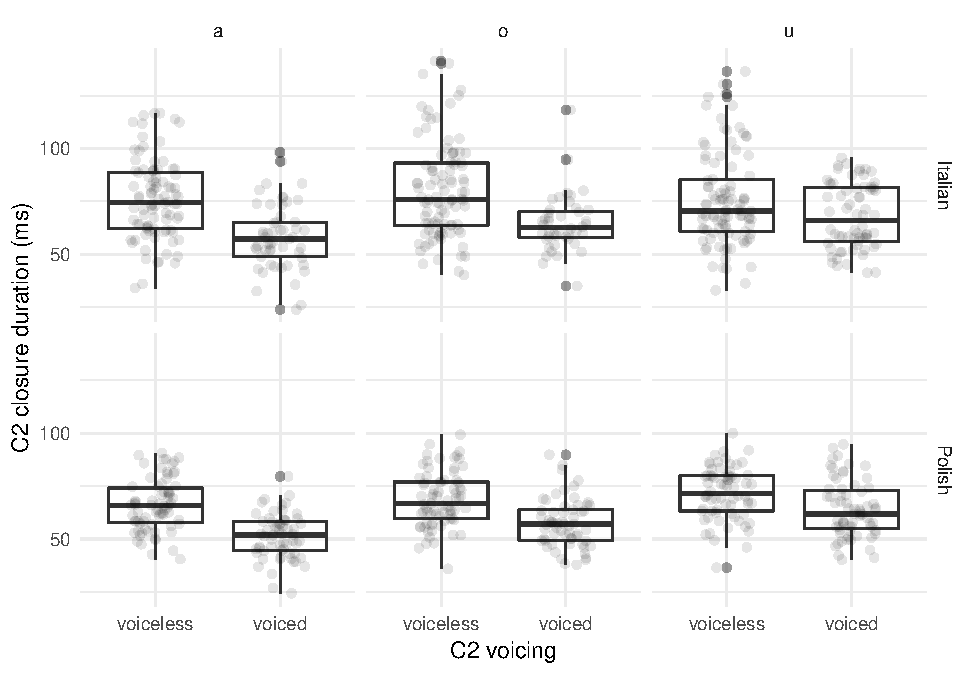
\includegraphics[width=\linewidth]{2018-relrel_files/figure-latex/Figure3} \caption{Raw data and boxplots of closure duration in milliseconds of voiceless and voiced stops in Italian (top row) and Polish (bottom row) when preceded by the vowels /a, o, u/}\label{f:Figure3}
\end{figure}

\Cref{f:Figure3} illustrates stop closure durations with boxplots and
individual raw data points. A pattern opposite to that with vowel
duration can be noticed: closure duration is shorter for voiced than for
voiceless stops. The closure of voiceless stops in Italian is 106.16 ms
long (SD = 27.08), while the voiced stops have a mean closure duration
of 117.66 ms (SD = 34.63). In Polish, the closure duration is 75.57 ms
(SD = 16.16) in voiceless stops and 83.11 ms (SD = 19.37) in voiced
stops. The difference in closure duration based on the raw means is
13.33 ms in Italian and 10.87 ms in Polish. The same model specification
as with vowel duration has been fitted with consonant closure duration
as the outcome variable. C2 voicing, C2 place, and speech rate are
significant. Stop closure is 16.5 ms shorter (SE = 3) if the stop is
voiced and 3.5 ms longer (SE = 1.5) if velar. Finally, faster speech
rates correlate with shorter closure durations (\(\hat{\beta}\) = -8.5
ms, SE = 1 ms).

\subsection{Vowel and closure
duration}\label{vowel-and-closure-duration}

\label{s:vcduration}

\begin{figure}
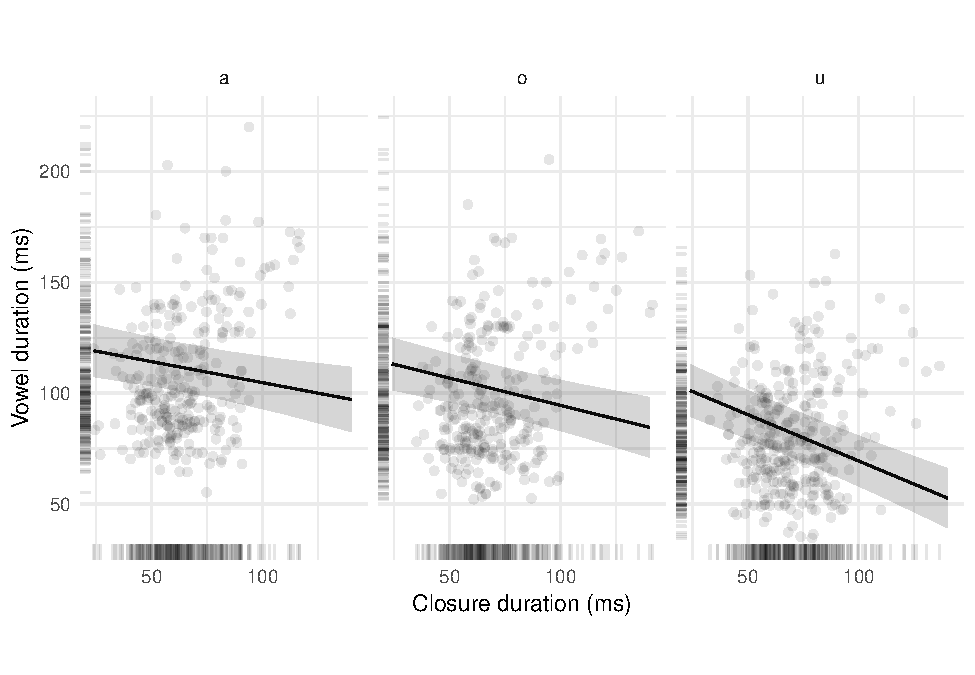
\includegraphics[width=\linewidth]{2018-relrel_files/figure-latex/Figure4} \caption{Raw data, estimated regression lines, and 95 per cent confidence intervals of the effect of closure duration on vowel duration for the vowels /a, o, u/ (from a mixed-effects model fitted to data pooled from Italian and Polish, see text for details)}\label{f:Figure4}
\end{figure}

A model addressing the relationship between vowel and stop closure
duration was fitted with the following terms and interactions: vowel
duration as the outcome variable; as fixed effects, closure duration,
vowel, speech rate (centred); all logical interactions between closure
duration, vowel, and speech rate; by-speaker and by-word random
intercepts. Closure duration has a significant effect on vowel duration
(\(\hat{\beta}\) = -0.19 ms, SE = 0.06 ms). The effect with /u/ is
greater than with /a/ and /o/ (\(\hat{\beta}\) = -0.23 ms, SE = 0.08
ms). In general, closure duration is inversely proportional to vowel
duration. However, such correlation is quite weak, as shown by the small
estimates. A 1 ms increase in closure duration corresponds to a
0.2--0.45 ms decrease in vowel duration. These estimates can be
interpreted in terms of percentages of compensation, which range between
20 and 45\%. Faster speech rates elicit a bigger effect than lower
speech rates, as indicated by the significant interaction between
closure duration and speech rate (\(\hat{\beta}\) = -0.2 ms, SE = 0.06
ms). The effect of the interaction is reduced when the vowel is /u/
(\(\hat{\beta}\) = 0.17 ms, SE = 0.08 ms). \Cref{f:Figure4} shows for
each vowel /a, o, u/ the individual data points and the regression lines
with 95\% confidence intervals extracted from the mixed-effects model.

\subsection{Word duration}\label{word-duration}

Words with a voiceless C2 are on average 393.72 ms long (SD = 79.05) in
Italian and 387.72 ms long (SD = 73.45) in Polish. Words with a voiced
stop have a mean duration of 357.07 ms (SD = 39.14) in Italian and
361.87 ms (SD = 38.51) in Polish. The following full and null models
were fitted to test the effect of C2 voicing on word duration. The full
model is made up of the following fixed effects: C2 voicing, C2 place,
vowel, language, and speech rate. The model also includes by-speaker and
by-word random intercepts, and a by-speaker random slope for C2 voicing.
The null model is the same as the full model with the exclusion of the
fixed effect of C2 voicing. The Bayes factor of the null against the
full model is 19. Thus, the null model (in which there is no effect of
C2 voicing, \(\beta\) = 0) is 19 times more likely under the observed
data than the full model. This indicates that there is positive evidence
for a null effect of C2 voicing on word duration.

\subsection{Release to release interval
duration}\label{release-to-release-interval-duration}

\begin{figure}
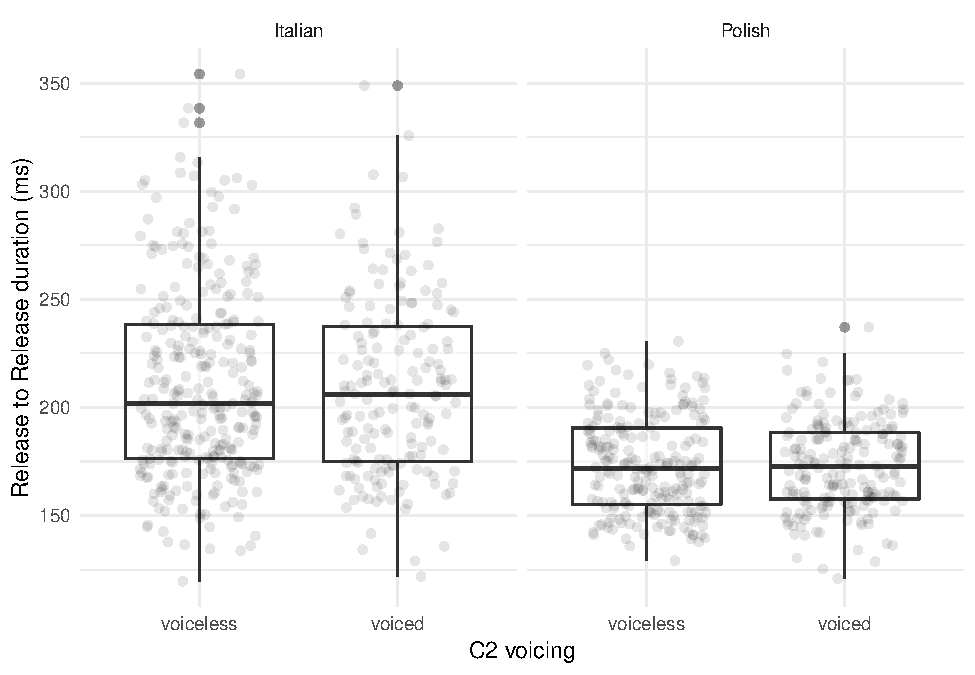
\includegraphics[width=\linewidth]{2018-relrel_files/figure-latex/Figure5} \caption{Raw data and boxplots of the duration in milliseconds of the release to release interval in Italian (left) and Polish (right) when C2 is voiceless or voiced}\label{f:Figure5}
\end{figure}

In \Cref{f:Figure5}, boxplots and raw data points show the duration of
the release to release interval in words with a voiceless vs.~a voiced
C2 stop, in Italian and Polish. It can be seen that the distributions,
medians, and quartiles of the durations in the voiceless and voiced
condition do not differ much in either language. In Italian, the mean
duration of the release to release interval is 209.88 ms (SD = 43.84) if
C2 is voiceless, and 208.6 ms (SD = 41.34) if voiced. In Polish, the
mean durations are respectively 173.13 (SD = 22.44) and 172.67 (SD =
20.47) ms. The specifications of the null and full models for the
release to release duration are the same as for word duration. The Bayes
factor of the null model against the full model is 21, which means that
the null model (without C2 voicing) is 21 times more likely than the
model with C2 voicing as a predictor. The Bayes factor suggests there is
strong evidence that duration of the release to release interval is not
affected by C2 voicing.

\section{Discussion}\label{discussion}

\label{s:discussion}

An exploratory study of articulatory and acoustic aspects of the effect
of consonant voicing on vowel duration in Italian and Polish has been
carried out to look for a possible source of such effect in speech
production. Only the results from the acoustic part of the study bear on
the main argument of this paper. The following sections discuss, in
turn, the results regarding the effect of voicing on vowel duration in
Italian and Polish and how the finding that the duration of the interval
between the two consecutive consonant releases in CV́CV words is
compatible with a compensatory temporal adjustment account of the
voicing effect. The section concludes by discussing the limitations and
open issues of this study.

\subsection{Voicing effect in Italian and
Polish}\label{voicing-effect-in-italian-and-polish}

The results of vowel duration and C2 voicing indicate that vowels are
longer when followed by voiced then when followed by voiceless stops
both in Italian and Polish. The estimated effect is around 16 ms when C2
is voiced for Italian. This value is not too far from the estimates of
previous works on this language
\citep{caldognetto1979, farnetani1986, esposito2002}, the range of which
is between 22 and 24 ms. The higher estimates of these studies compared
to the one here could be related to differences in experimental design,
or Type M (magnitude) errors due to low statistical power in previous
studies (see \citealt{kirby2018}). The estimate of the effect of voicing
on C2 closure duration is around -18 ms. Crucially, the effect of
voicing on vowel and closure duration have similar magnitudes, but
opposite signs. These results suggest a compensatory mechanism between
vowel and closure duration.

Furthermore, the effect of voicing on the duration of Italian /u/ is
smaller than with /a/ and /o/ (about 3 vs.~16 ms respectively), a fact
already observed by \citealt{ferrero1978}. While it is not clear why the
duration of this particular vowel should not be affected by C2 voicing,
the data reported here indicate that the magnitude of the difference in
closure duration when the preceding vowel is /u/ is smaller than with
/a/ and /o/ (about 7 vs.~17 ms respectively). If vowel duration
compensates for closure duration, then a smaller difference in closure
duration should correspond to a small difference in vowel duration, as
the estimates seem to suggest.

The interpretation of the Polish results is less straightforward.
Previous studies found either no voicing effect or a small effect in
Polish (3.5--4.5 ms). In particular, \citet{malisz2008} say that the
effect seems to be very idiosyncratic in the 40 speakers of their
analysis. The estimated effect found in the 6 Polish speakers of the
present study is 10.54 ms, and the difference based on the means of the
raw vowel durations is 7.5 ms. Recall, however, that the interaction
between language and C2 voicing (which gives the estimate of 10.54) is
not significant (see the full model summary in \Cref{tab:vow-table}). It
is likely, though, that the non-significance might be related to low
power. Indeed, only 6 Polish speakers have been recorded, against 11
speakers of Italian. The raw mean difference of 7.5 ms in
Polish---although still higher than what found in previous
studies---might be more informative in this case.

More specifically, when one compares the raw mean duration differences
of vowels with the raw mean duration differences of consonant closures,
a pattern can be seen. The mean differences of Italian vowels and
closures (11.5 and 13.33, respectively) are bigger than those of Polish
(7.54 and 10.87), although by a small amount (about 3 ms). It is
plausible that the smaller effect of C2 voicing on preceding vowel
duration in Polish is related to the smaller effect on closure duration,
if we assume a temporal mechanism of compensation between the closure
and the vowel. Of course these patterns need to be confirmed with a more
balanced sample of Italian and Polish speakers.

\subsection{Compensatory temporal
adjustment}\label{compensatory-temporal-adjustment}

Vowels followed by voiced stops are long, while vowels followed by
voiceless stops are short. The closure duration of voiced stops is short
compared to that of voiceless stops. There seems to be an inverse
relationship between vowel duration and closure duration, by which a
long vowel entails a short closure (and vice versa), and a short vowel
entails a long closure (and vice versa).

The data and statistical analyses of this exploratory study suggest that
the duration of the interval between the releases of two consecutive
consonants in CV́CV words (the release to release interval) is not
affected by the phonological voicing of the second consonant (C2) in
Italian and Polish. In accordance with a compensatory temporal
adjustment account \citep{slis1969, lehiste1970}, the difference in
vowel duration before voiceless vs.~voiced stops can be seen as the
outcome of differences in stop closure duration. In other words, the
timing of the (acoustic) closure onset of C2 within the temporally
stable release to release interval determines the duration of the
preceding vowel. An earlier closure onset relative to the onset of the
preceding vowel (like in the case of voiceless stops) causes the vowel
to be shorter. On the other hand, a later closure onset (like with
voiced stops) produces a longer vowel. Note that the term `temporal
stability' (and `temporally stable') as used here means that the
underlying statistical distribution of the interval duration is stable
\emph{across contexts of C2 voicing}. No specific statement is implied
about the variance of the duration around the mean, across or within
phonological contexts. \Cref{f:compensatory} illustrates the
compensatory mechanism.

\begin{figure}
  \centering
  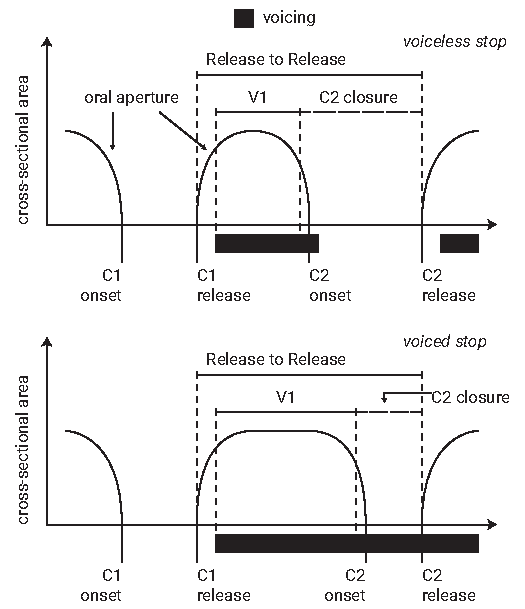
\includegraphics{img/Figure6.pdf}
  \caption{A schematic representation of the oral cavity cross-sectional area, as inferred from acoustics. Design based on \citet{esposito2002}. The top panel shows a CV́C sequence with a voiceless C2, the bottom panel with a voiced C2. Oral cavity aperture (on the \textit{y}-axis, as the inverse of oral constriction) through time (on the \textit{x}-axis) is represented by the black line. Lower values represent a more constricted oral tract (a contoid configuration), while higher values indicate a more open oral tract (a vocoid configuration). The black bars below the time axis represent voicing (vocal fold vibration). Various landmarks and intervals are indicated in the schematic}
  \label{f:compensatory}
\end{figure}

The invariance of the release to release interval allows us to refine
the logistics of the compensatory account by narrowing the scope of the
temporal adjustment action. A limitation of this account, as proposed by
\citet{slis1969} and \citet{lehiste1970}, is the lack of a precise
identification of the word-internal mechanics of compensation. As
already discussed in \Cref{s:intro}, it is not clear why the adjustment
should target the preceding stressed vowel, rather then the following
unstressed vowel or any other segment in the word. Since the release to
release interval includes just the vocoid gesture between the release of
C1 and the onset of the closure of C2 and the consonant closure, it
follows that differences in closure duration must be reflected in
differences in the duration of the preceding vocoid. It is worth noting,
though, that other accounts---which could be compatible with other
aspects of production and perception---aren't ultimately ruled out. For
example, perceptual factors might play a role in the enhancement of the
effect (see \citealt{kingston1994}, \citealt{port1982}, and
\citealt{luce1985}). Other perceptual explanations of the voicing effect
have been proposed in \citet{javkin1976} and \citet{kluender1988}.

Under an account of temporal compensation, the voicing effect can be
interpreted as a by-product of gestural phasing, rather then a
consequence of intrinsic features of voicing \emph{per se}. The temporal
stability of the release to release interval across voicing contexts
allows us to refine the compensatory mechanism by providing a temporal
anchor. On the other hand, it is important to note that the release to
release interval should not necessarily have a special status in such
compensatory account, but rather can be used as a proxy to the
understanding of a full gestural mechanism of compensation. Indeed, the
temporal stability of this interval should be derivable from a theory of
gestural phasing, rather than one that simply states that the interval
is stable across voicing contexts. While beyond the scope of this paper,
work on the gestural coordination of sequences besides the traditional
syllable might reveal a principled organisation that results in the
temporal patterns observed in this study.

\subsection{Limitations and future
work}\label{limitations-and-future-work}

The generalisations put forward in this paper strictly apply to
disyllabic words with a stressed vowel in the first syllable, flanked by
single stops. First, it is possible that the pattern found in this
context does not occur in sequences including an unstressed vowel. For
example, it is known that the difference in closure duration between
voiceless and voiced stops is not stable when the stops precede a
stressed vowel, although vowels preceding pre-stress stops have slightly
different durations \citep{davis1989}. According to the interpretation
given here, the absence of differences in closure duration should
correspond to the absence of differences in vowel duration. Second, it
is known that the magnitude of the effect of voicing is modulated by
other prosodic characteristics, like the number of syllables in the
word, presence/absence of focus, and position within the sentence
\citep{sharf1962, klatt1973, laeufer1992, de-jong2004}. Third, the
constraints on experimental material enforced by the use of ultrasound
tongue imaging have been previously mentioned in \Cref{s:materials}.
Given these constraints, temporal information from other vowels (like
front vowels), places and manners of articulation is a desideratum. Data
from different contexts and different languages is thus needed to assess
the generality of the claims put forward in this paper.

Another issue is the interaction of the temporal compensation and speech
rate. The magnitude of compensation between vowel and closure duration
found in \citet{de-jong1991} and here is somewhat small (between 12\%
and 40\%). Ideally, given the temporal stability of the release to
release interval relative to C2 voicing, the compensation rates should
approximate 100\%. However, it is possible that the correlation between
vowel and closure duration is modulated in complex ways by the
individual effects of speech rate on the vowel and the closure. For
example, \citet{ko2018} finds that the vowel/closure ratio differs
depending on speaking rate and that there is an interaction between the
voicing of the consonant and speaking rate. When the consonant is
voiceless, the vowel/closure ratio is smaller when speaking rate is
slow, while slow speaking rate induces larger vowel/closure values when
the consonant is voiced. Experimental work is required which addresses
the differential effect of speaking rate on vowel and consonant
closures, and how these interact with a possible compensatory mechanism.

The compensatory temporal adjustment account presented here extends to
other durational effects discussed in the literature. In particular, the
account bears predictions on the direction of the durational difference
led by phonation types different from voicing, like aspiration and
ejection. For example, the mix of results with regard to the effect of
aspiration \citep{durvasula2012} suggests that the conditions for a
temporal adjustment might differ across the contexts and languages
studied. In light of the results in \citet{begus2017}, future studies
will also have to investigate the durational invariance of speech
intervals in relation to a variety of phonation contrasts.

\section{Conclusions}\label{conclusions}

The results of an exploratory study on the effect of voicing on vowel
duration are congruent with a compensatory temporal adjustment account
of such effect. Acoustic data from seventeen speakers of Italian and
Polish show that the temporal distance between two consecutive stop
releases is not affected by the voicing of the second stop in CV́CV
words. The temporal invariance of the release to release interval,
together with a difference in stop closure duration of voiceless and
voiced stops, causes vowels to be shorter when followed by voiceless
stops (which have a long closure) and longer when followed by voiced
stops (the closure of which is short). Future work will need to
investigate further aspects of the patterns found in this study, with a
particular focus on the effects of different segmental and prosodic
structures and different laryngeal contrasts on the release to release
interval.

\section{Acknowledgements}\label{acknowledgements}

I am grateful to Ricardo Bermúdez-Otero and Patrycja Strycharczuk for
their immense support and patience in providing feedback on this
project. I also want to thank the audience at the 16th Laboratory
Phonology conference (LabPhon16) for their input, and Kenneth de Jong
for comments on an early draft of this paper. Thanks also go to my
colleagues at the Phonetics Laboratory of the University of Manchester,
who provided help in different ways. Any remaining errors are my own.
This project has been funded by the School of Arts, Languages, and
Cultures Graduate School at the University of Manchester.

\appendix

\section{Output of statistical
models}\label{output-of-statistical-models}

\label{a:stats}

See \Cref{tab:vow-table}, \Cref{tab:clo-table}, and
\Cref{tab:vow-clo-table}.

\begin{table}

\caption{\label{tab:vow-table}Summary of the linear mixed-effects model fitted to vowel duration (see \Cref{s:vduration})}
\centering
\fontsize{8}{10}\selectfont
\begin{tabular}[t]{lrrrrrrrl}
\toprule
Predictor & Estimate & SE & CI low & CI up & df & t-value & p-value & < α\\
\midrule
Intercept & 118.06 & 4.94 & 108.38 & 127.74 & 23.89 & 23.91 & 0.00 & *\\
Voicing = voiced & 16.28 & 4.42 & 7.62 & 24.95 & 15.38 & 3.68 & 0.00 & *\\
Vowel = /o/ & -7.50 & 3.93 & -15.21 & 0.21 & 10.31 & -1.91 & 0.08 & \\
Vowel = /u/ & -25.71 & 3.94 & -33.44 & -17.98 & 10.43 & -6.52 & 0.00 & *\\
Lang = Polish & -24.05 & 7.83 & -39.40 & -8.69 & 22.38 & -3.07 & 0.01 & *\\
Place = velar & -7.95 & 1.63 & -11.15 & -4.75 & 10.99 & -4.87 & 0.00 & *\\
Speech rate & -16.23 & 1.26 & -18.69 & -13.77 & 854.63 & -12.91 & 0.00 & *\\
Voiced × /o/ & 2.09 & 5.54 & -8.77 & 12.96 & 10.18 & 0.38 & 0.71 & \\
Voiced × /u/ & -13.09 & 5.56 & -23.99 & -2.20 & 10.30 & -2.36 & 0.04 & *\\
Voiced × Polish & -5.73 & 6.61 & -18.69 & 7.23 & 18.00 & -0.87 & 0.40 & \\
/o/ × Polish & -2.50 & 5.66 & -13.60 & 8.60 & 11.09 & -0.44 & 0.67 & \\
/u/ × Polish & 1.12 & 5.68 & -10.01 & 12.26 & 11.23 & 0.20 & 0.85 & \\
Voiced × /o/ × Polish & -6.16 & 8.00 & -21.85 & 9.53 & 11.06 & -0.77 & 0.46 & \\
Voiced × /u/ × Polish & 6.40 & 8.03 & -9.34 & 22.13 & 11.19 & 0.80 & 0.44 & \\
\bottomrule
\end{tabular}
\end{table}

\begin{table}

\caption{\label{tab:clo-table}Summary of the linear mixed-effects model fitted to closure duration (see \Cref{s:cduration})}
\centering
\fontsize{8}{10}\selectfont
\begin{tabular}[t]{lrrrrrrrl}
\toprule
Predictor & Estimate & SE & CI low & CI up & df & t-value & p-value & < α\\
\midrule
Intercept & 73.25 & 4.28 & 64.86 & 81.63 & 22.38 & 17.11 & 0.00 & *\\
Voicing = voiced & -17.70 & 4.06 & -25.66 & -9.74 & 18.63 & -4.36 & 0.00 & *\\
Vowel = /o/ & 3.75 & 3.26 & -2.64 & 10.14 & 9.43 & 1.15 & 0.28 & \\
Vowel = /u/ & -1.91 & 3.27 & -8.32 & 4.50 & 9.56 & -0.58 & 0.57 & \\
Lang = Polish & -7.03 & 6.82 & -20.40 & 6.34 & 20.82 & -1.03 & 0.31 & \\
Place = velar & 3.80 & 1.38 & 1.08 & 6.51 & 10.94 & 2.74 & 0.02 & *\\
Speech rate & -7.86 & 1.13 & -10.08 & -5.64 & 488.55 & -6.94 & 0.00 & *\\
Voiced × /o/ & 1.91 & 4.88 & -7.65 & 11.47 & 11.80 & 0.39 & 0.70 & \\
Voiced × /u/ & 10.88 & 4.79 & 1.50 & 20.27 & 10.97 & 2.27 & 0.04 & *\\
Voiced × Polish & 2.30 & 6.07 & -9.59 & 14.19 & 19.83 & 0.38 & 0.71 & \\
/o/ × Polish & -1.04 & 4.67 & -10.19 & 8.10 & 9.94 & -0.22 & 0.83 & \\
/u/ × Polish & 6.94 & 4.68 & -2.24 & 16.12 & 10.09 & 1.48 & 0.17 & \\
Voiced × /o/ × Polish & 1.36 & 6.84 & -12.04 & 14.77 & 11.44 & 0.20 & 0.85 & \\
Voiced × /u/ × Polish & -3.08 & 6.77 & -16.35 & 10.20 & 11.01 & -0.45 & 0.66 & \\
\bottomrule
\end{tabular}
\end{table}

\begin{table}

\caption{\label{tab:vow-clo-table}Summary of the linear mixed-effects model for testing the correlation between vowel and closure duration (see \Cref{s:vcduration})}
\centering
\fontsize{8}{10}\selectfont
\begin{tabular}[t]{lrrrrrrrl}
\toprule
Predictor & Estimate & SE & CI low & CI up & df & t-value & p-value & < α\\
\midrule
Intercept & 123.62 & 6.76 & 110.36 & 136.87 & 56.24 & 18.27 & 0.00 & *\\
Closure dur. & -0.19 & 0.06 & -0.32 & -0.06 & 816.53 & -2.93 & 0.00 & *\\
Vowel = /o/ & -4.54 & 6.31 & -16.90 & 7.82 & 127.46 & -0.72 & 0.47 & \\
Vowel = /u/ & -12.47 & 6.40 & -25.00 & 0.07 & 134.64 & -1.95 & 0.05 & \\
Speech rate & -5.16 & 4.28 & -13.55 & 3.23 & 827.04 & -1.21 & 0.23 & \\
Closure × /o/ & -0.06 & 0.08 & -0.22 & 0.10 & 829.38 & -0.71 & 0.48 & \\
Closure × /u/ & -0.23 & 0.08 & -0.39 & -0.07 & 831.49 & -2.82 & 0.00 & *\\
C2 closure × sp. rate & -0.20 & 0.06 & -0.32 & -0.08 & 826.97 & -3.18 & 0.00 & *\\
/o/ × sp. rate & -3.75 & 5.19 & -13.92 & 6.42 & 819.79 & -0.72 & 0.47 & \\
/u/ × sp. rate & -10.13 & 5.50 & -20.91 & 0.64 & 822.55 & -1.84 & 0.07 & \\
Closure × /o/ × sp. rate & 0.09 & 0.07 & -0.06 & 0.23 & 820.74 & 1.17 & 0.24 & \\
Closure × /u/ × sp. rate & 0.17 & 0.08 & 0.01 & 0.32 & 823.88 & 2.14 & 0.03 & *\\
\bottomrule
\end{tabular}
\end{table}

\section{Socio-linguistic information of
participants}\label{socio-linguistic-information-of-participants}

\label{a:socioling}

See \Cref{t:socio}.

\ctable[caption = Participants' sociolinguistic information. The column 'Spent most time in' gives the city in which the participant spent most of their life. The last column ('> 6 mo') indicates whether the participant has spent more than 6 months abroad,
label = t:socio,
width=\textwidth,
star,
doinside = \scriptsize
]{llll>{\raggedright}p{3cm}l>{\raggedright}p{2cm}l}{}{
\FL
ID & Age & Sex    & Native L & Other Ls& City of birth & Spent most time in & > 6 mo \ML
IT01 & 29 & Male   & Italian & English, Spanish                          & Verbania            & Verbania        & Yes \NN
IT02 & 26 & Male   & Italian & Friulian, English, Ladin-Venetan          & Udine               & Tricesimo & Yes \NN
IT03 & 28 & Female & Italian & English, German                           & Verbania            & Verbania        & No  \NN
IT04 & 54 & Female & Italian & Calabrese                                 & Verbania            & Verbania        & No  \NN
IT05 & 28 & Female & Italian & English                                   & Verbania            & Verbania        & No  \NN
IT09 & 35 & Female & Italian & English                                   & Vignola & Vignola         & Yes \NN
IT11 & 24 & Male   & Italian & English                                   & Monza               & Monza           & Yes \NN
IT12 & 26 & Male   & Italian & English                                   & Rome               & Rome           & Yes \NN
IT13 & 20 & Female & Italian & English, French, Arabic, Farsi            & Ancona              & Chiaravalle     & Yes \NN
IT14 & 32 & Male & Italian & English, Spanish & Frosinone & Frosinone & Yes \NN
PL02 & 32 & Female & Polish  & English, Norwegian, French, German, Dutch & Koło                & Poznań          & Yes \NN
PL03 & 26 & Male   & Polish  & Russian, English, French, German          & Nowa Sol            & Poznań          & Yes \NN
PL04 & 34 & Female & Polish  & Spanish, English, French                  & Warsaw              & Warsaw          & No  \NN
PL05 & 42 & Male   & Polish  & English, French                           & Przasnysz           & Warsaw        & No  \NN
PL06 & 33 & Male   & Polish  & English                                   & Zgierz              & Zgierz          & Yes \NN
PL07 & 32 & Female & Polish  & English, Russian                          & Bielsk Podlaski     & Bielsk Podlaski & Yes \LL
}

\section{Target words}\label{target-words}

\label{a:targets}

See \Cref{t:targets}.

\ctable[caption = Target words. Asterisks indicate real words,
label = t:targets,
star,
doinside = \footnotesize
]{lllllll}{}{
\FL
Italian   &        &      & \hspace{0.5cm} & Polish &      &      \NN
\cmidrule{1-3}\cmidrule{5-7}
pata      & poto*  & putu & & pata   & poto & putu \NN
pada      & podo   & pudu & & pada*  & podo & pudu \NN
paca*     & poco*  & pucu & & paka*  & poko & puku \NN
paga*     & pogo   & pugu & & paga   & pogo & pugu \LL
}

\bibliography{linguistics}


\end{document}
